
\documentclass[manuscript,screen,review, nonacm]{acmart}

\usepackage{graphicx}
\usepackage{float}


%%
%% end of the preamble, start of the body of the document source.
\begin{document}

%%
%% The "title" command has an optional parameter,
%% allowing the author to define a "short title" to be used in page headers.
\title{Exploratory Data Analysis}

%%
%% The "author" command and its associated commands are used to define
%% the authors and their affiliations.
%% Of note is the shared affiliation of the first two authors, and the
%% "authornote" and "authornotemark" commands
%% used to denote shared contribution to the research.
\author{Harvey Kwong}
\email{harveykw@buffalo.edu}
\author{Jacob DeRosa}
\email{jderosa3@buffalo.edu}
\affiliation{%
  \institution{University at Buffalo}
  \city{Buffalo}
  \state{New York}
  \country{USA}
}


\maketitle

\section{Introduction and Problem Statement}

    The rise of antibiotic resistant infections poses a significant challenge to global public health. Due to rapidly increasing resistance to 
available treatments and its difficulty to be detected, gonorrhoea is one of the most concerning pathogens in recent history. This project focuses on predicting antibiotic resistance 
in Neisseria gonorrhoeae, the bacteria responsible for gonorrhoea, using subsets of its DNA sequences as predictive features. 
The primary objective of this project is to explore the relationship between bacterial DNA segments and 
resistance patterns, and to identify key genetic markers that could possibly predict resistance. By performing data 
cleaning and exploratory data analysis on a dataset containing DNA sequences and resistance outcomes, 
we aim to address the following question: Which DNA segments are most associated with antibiotic resistance? 

    This project’s contribution is very important as it helps to clarify biological data, making it easier for 
future studies to focus on effective solutions. By gaining a deeper understanding of the data and identifying 
key variables, this project serves as a step towards more advanced research on antibiotic resistance.

\section{Data Sources}

    We utilized the "Predicting antibiotic resistance in gonorrhoea" dataset from Kaggle: \\
    (https://www.kaggle.com/datasets/nwheeler443/gono-unitigs/data). \\


\section{Data Cleaning/Processing}

    We have completed 11 total unique data cleaning and processing steps:

    \begin{itemize}
        \item[1.] Removed all rows that were NaN in our target label field - Our target labels we aim to predict down the line
        are: azm\_sr, cfx\_sr, and cip\_sr. If the labels were missing, then we cannot use that row.

        \item[2.] Removed unused columns - The dataset contained multiple types of resistances. Because we only focus on 3, the rest can
        can be discarded safely. We also use this step to remove the year column. This is because these features will have no impact on our results.

        \item[3.] Removed duplicate rows - Duplicate rows have the ability to skew our data. As such we removed all duplicate rows.
        
        \item[4.] Removed all symbols - Our data are either numerical or categorical (text). There is no need for symbols which will
        only cause problems down the line.

        \item[5.] Turned all non-numeric data within numerical columns into NaN, to be processed later - We have columns that are
        supposed to contain only numerical data, however, there are rows where there are letters in there. In this step, we turn them
        into NaN. This is because we will impute all NaNs later on.

        \item[6.] Cast all numerical columns into float32 - To establish precision.
        \item[7.] One hot encode categorical columns - Some columns such as "country" should be one hot encoded as we would want
        numerical representations of all our data for modelling.
        \item[8.] Handle "Beta.lactamase" special case - It is a numerical column but appears to be categorical in nature. As such
        we cannot impute missing values like with the other numerical columns. In this step, we set all missing entries to 0, and
        one hot encode the feature like with the non-numerical columns.
        \item[9.] Split dataframe into Train/Test - We will be doing additional data processing such as normalization and imputation later on.
        As such, we need to make the split beforehands for good practice in preventing leakage.
        \item[10.] Impute missing values in numerical columns - For every NaN in the numerical columns, we use skew based imputation to
        generate a new value that can substitute the NaN. This ensures that we have enough data to work with as we do not need to discard the entire row.
        \item[11.] Normalize all numerical columns - We do columnwise normalization on numerical columns. This is to ensure that we do not have extremely
        large values. This will preserve consistency in the distribution while being easier for the model to interpret. Normalization also prevents numerical instability when training.

    \end{itemize}



\section{Exploratory Data Analysis}

\begin{itemize}
    \item[1.] Calculate what percentage of rows correspond to specific labels - We found that 0.1779 of samples have resistance to azm, 
    0.0911 of samples have resistance to cfx, and 0.5353 of samples have resistance to cip. This gives us a basic idea of how difficult it may be for the model to find a relationship between unitig based features and their respective strain.
    \item[2.] We calculated the mean, median, and mode, standard deviation, and variance for all numerical columns. 
    Calculating the mean, median, mode, standard deviation, and variance for numerical columns is important for understanding the tendencies, spread, and variability of the data,
    which can help with data analysis and modeling. - See table 1.
    \begin{table}[H]
        \centering
        \begin{tabular}{|l|l|l|l|l|}
        \hline
        \textbf{Column}       & \textbf{Mean}    & \textbf{Median}  & \textbf{Std}     & \textbf{Variance} \\ \hline
        Azithromycin          & 0.000556         & 7.02e-05         & 0.0200           & 0.000401          \\ \hline
        Ciprofloxacin         & 0.0697           & 0.0697           & 0.0816           & 0.00666           \\ \hline
        Ceftriaxone           & 0.00107          & 1e-06            & 0.0296           & 0.000876          \\ \hline
        Cefixime              & 0.1855           & 0.121            & 0.2267           & 0.0514            \\ \hline
        Tetracycline          & 0.0571           & 0.0571           & 0.0709           & 0.00502           \\ \hline
        Penicillin            & 0.1447           & 0.1447           & 0.1562           & 0.0244            \\ \hline
        NG\_MAST              & 0.2790           & 0.2576           & 0.2342           & 0.0548            \\ \hline
        Group                 & 0.3658           & 0.2755           & 0.2952           & 0.0871            \\ \hline
        azm\_mic              & 0.00743          & 0.00036          & 0.0583           & 0.00340           \\ \hline
        cip\_mic              & 0.1162           & 0.0469           & 0.1694           & 0.0287            \\ \hline
        cro\_mic              & 0.0149           & 0.00738          & 0.0413           & 0.00170           \\ \hline
        cfx\_mic              & 0.00765          & 0.00275          & 0.0270           & 0.000727          \\ \hline
        tet\_mic              & 0.0306           & 0.0306           & 0.0579           & 0.00335           \\ \hline
        pen\_mic              & 0.0223           & 0.0223           & 0.0390           & 0.00152           \\ \hline
        log2\_azm\_mic        & 0.2895           & 0.2895           & 0.1443           & 0.0208            \\ \hline
        log2\_cip\_mic        & 0.4923           & 0.4923           & 0.3130           & 0.0980            \\ \hline
        log2\_cro\_mic        & 0.4409           & 0.4409           & 0.1313           & 0.0172            \\ \hline
        log2\_cfx\_mic        & 0.3676           & 0.3489           & 0.1176           & 0.0138            \\ \hline
        log2\_tet\_mic        & 0.5267           & 0.5267           & 0.1011           & 0.0102            \\ \hline
        log2\_pen\_mic        & 0.5359           & 0.5356           & 0.0936           & 0.00877           \\ \hline
        \end{tabular}
        \caption{Summary Statistics for Antibiotic Resistance Data}
    \end{table}
    \item[3.] Univariate Analysis - We examined the feature distribution for each numerical column. This gives us crucial insights into individual feature behavior 
    and will help in selecting appropriate preprocessing and model techniques. - See figure 1.
            \begin{figure}[H]
                \centering
                \vspace{-10pt}
                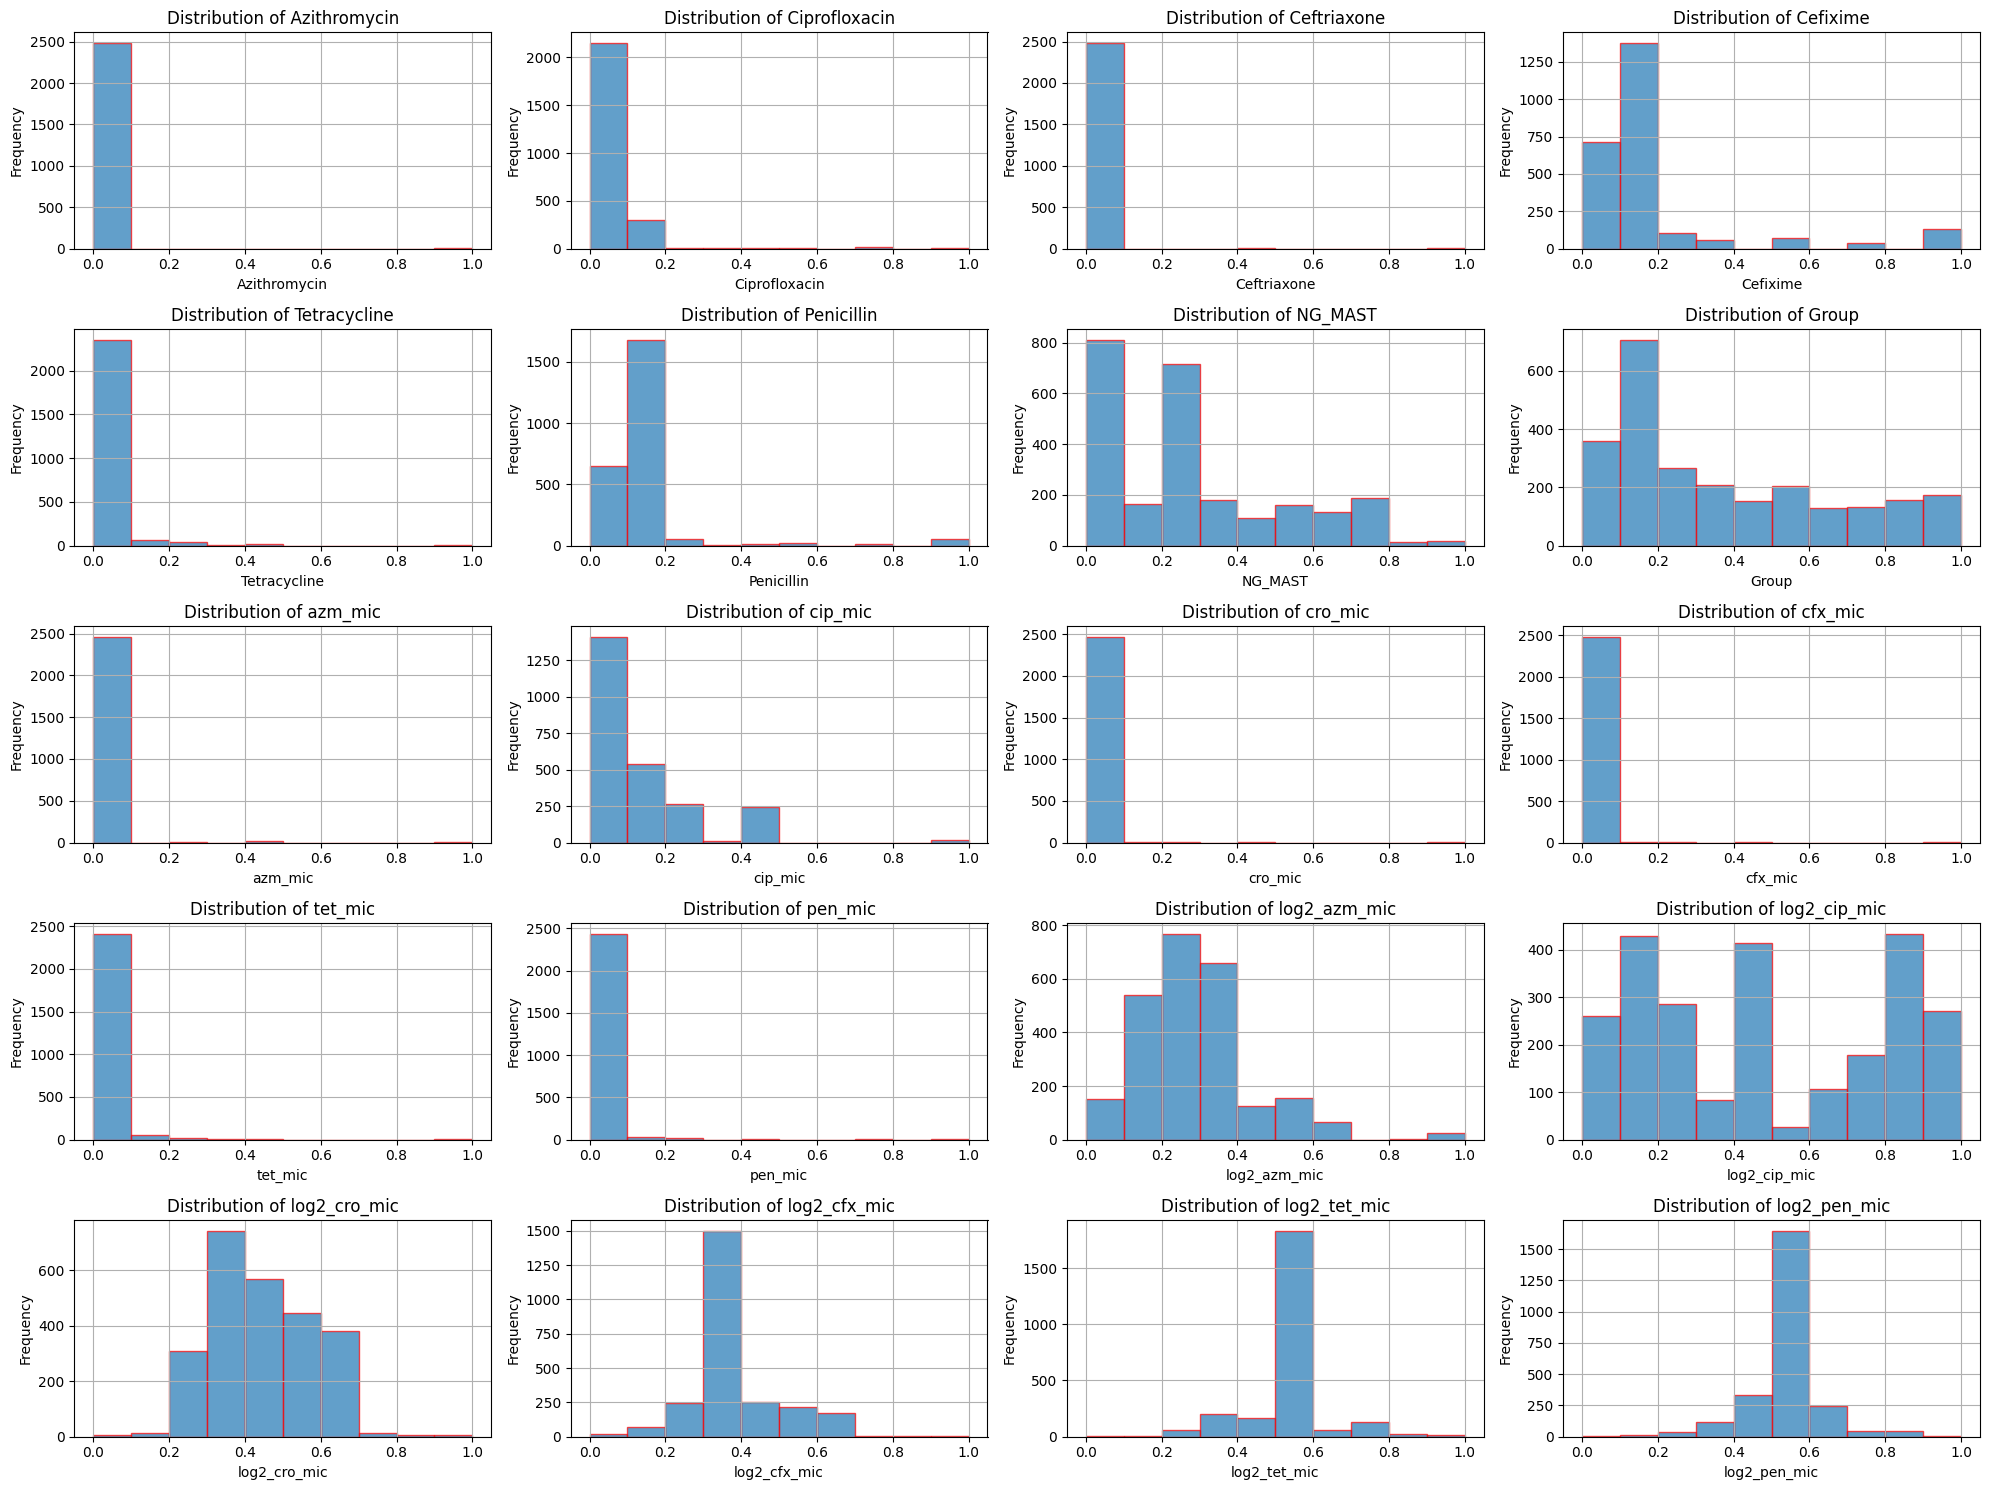
\includegraphics[width=0.7\textwidth]{figures/univar.png}
                \caption{Univariate analysis.}
                \vspace{-10pt}
            \end{figure}

    \item[4.] Multivariate Analysis - We examine each feature with respect to the labels we are interested in. This helps in identifying potential correlations and
    patterns that can be useful for predicting the labels, and gives insights into the relationships between variables and the targets. - See figure 2.
            \begin{figure}[H]
                \centering
                \vspace{-10pt}
                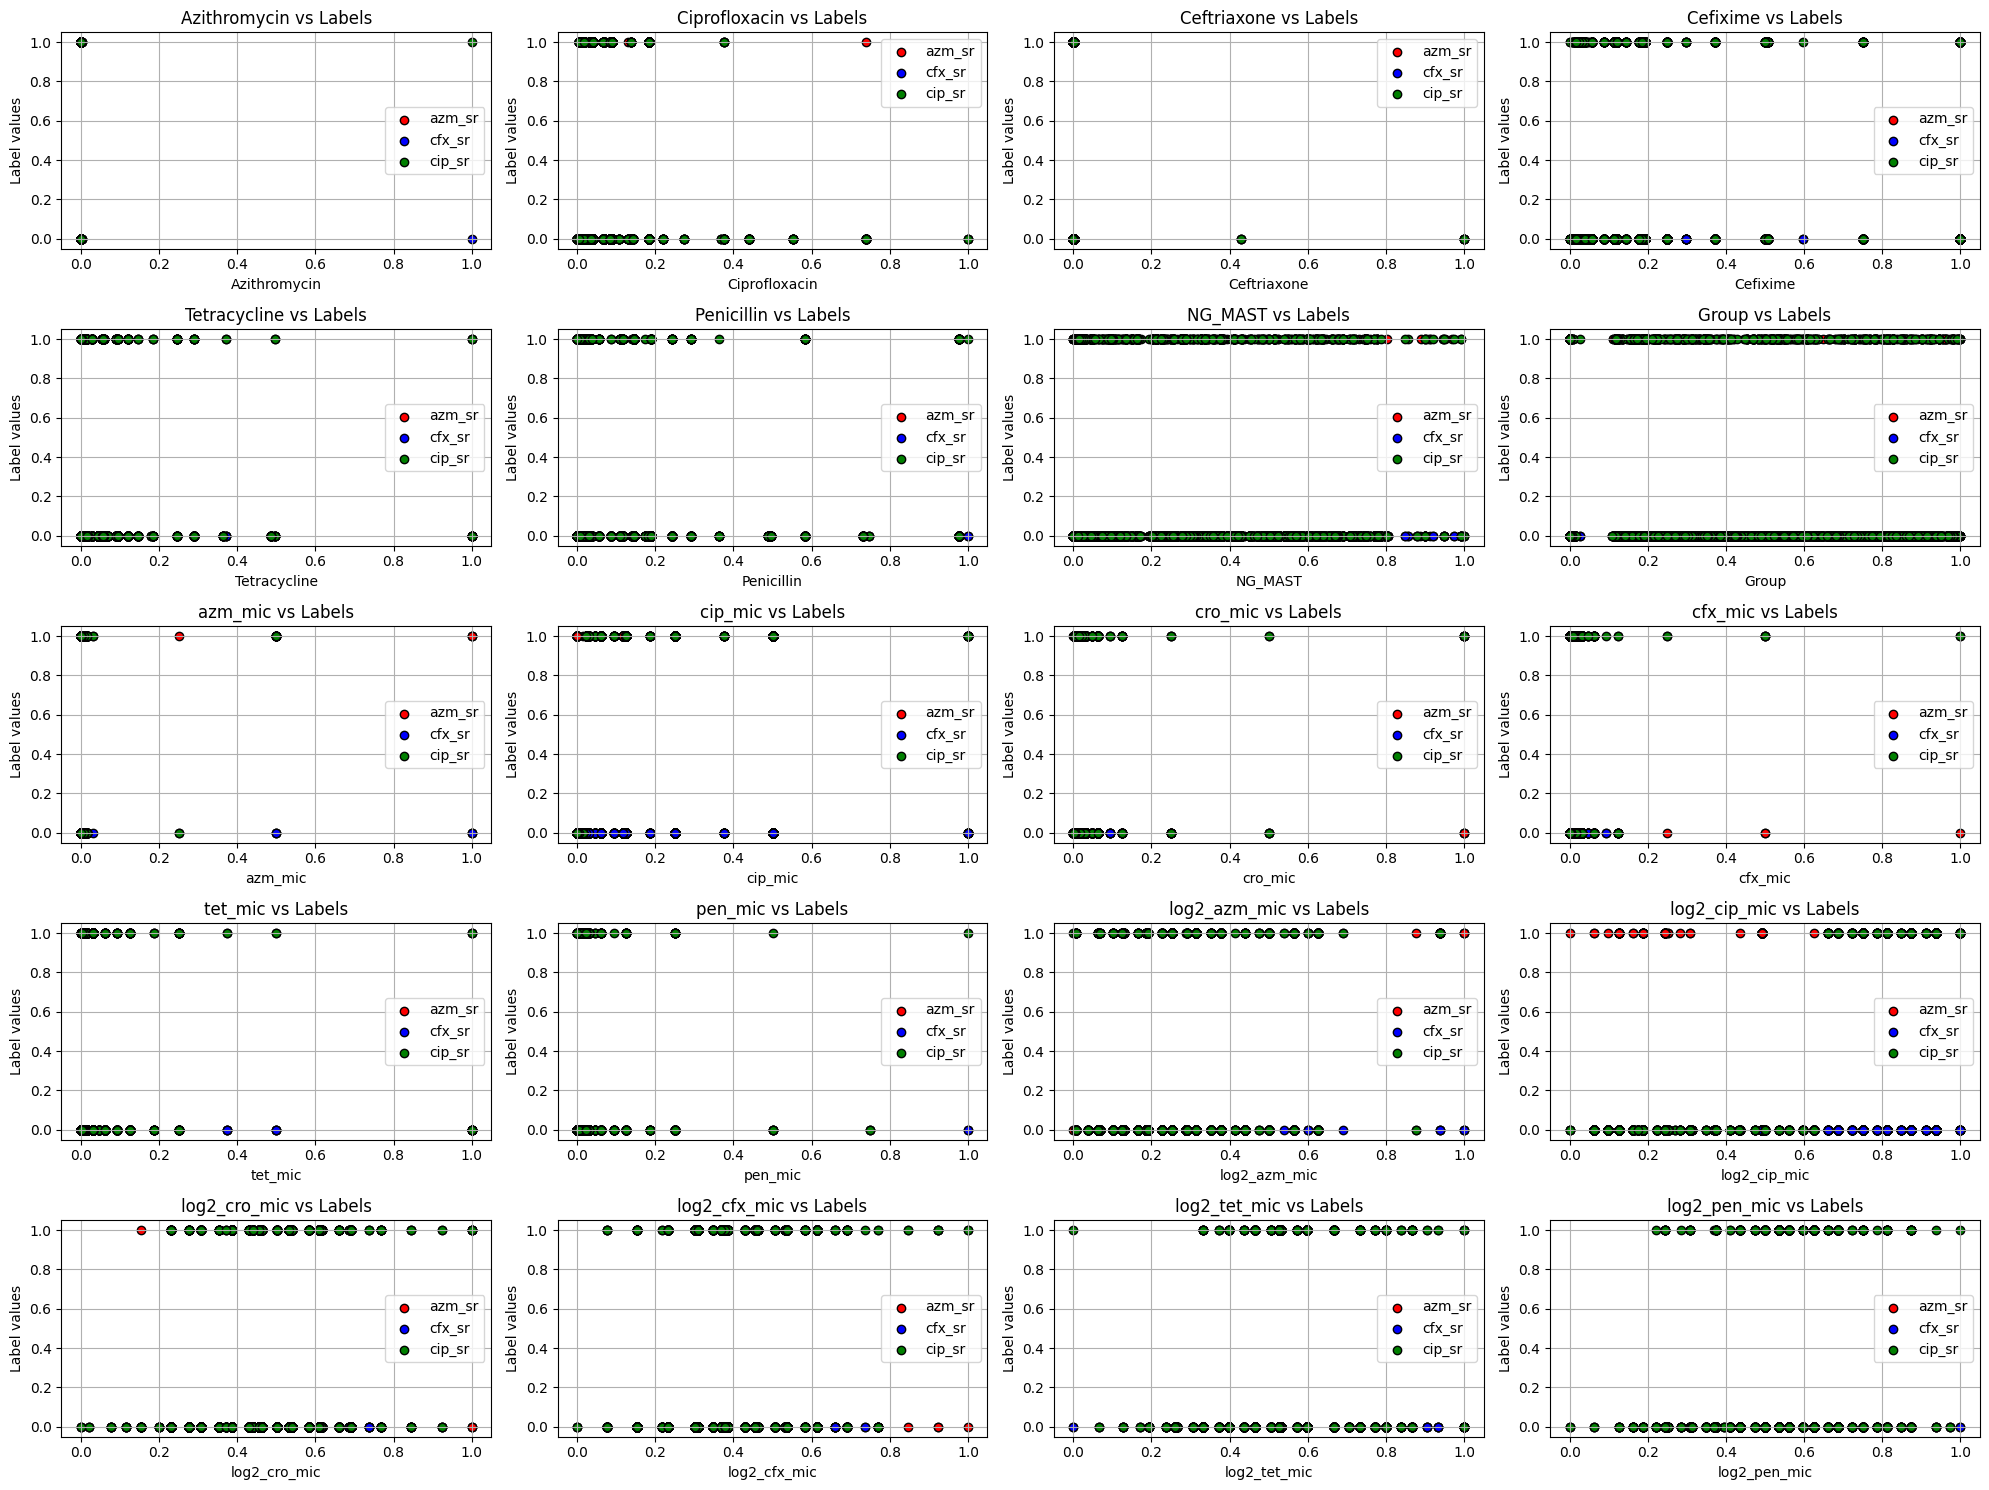
\includegraphics[width=0.7\textwidth]{figures/multivar.png}
                \caption{Multivariate analysis.}
                \vspace{-10pt}
            \end{figure}

    \item[5.] Correlation Analysis - We determine the Pearson correlation of each feature with respect to the labels. By quantifying the strength and direction of the relationships between features and labels, we can effectively display these correlations. This helps identify what features are the most influential
    feature on our target labels - See figure 3.
            \begin{figure}[H]
                \centering
                \vspace{-15pt}
                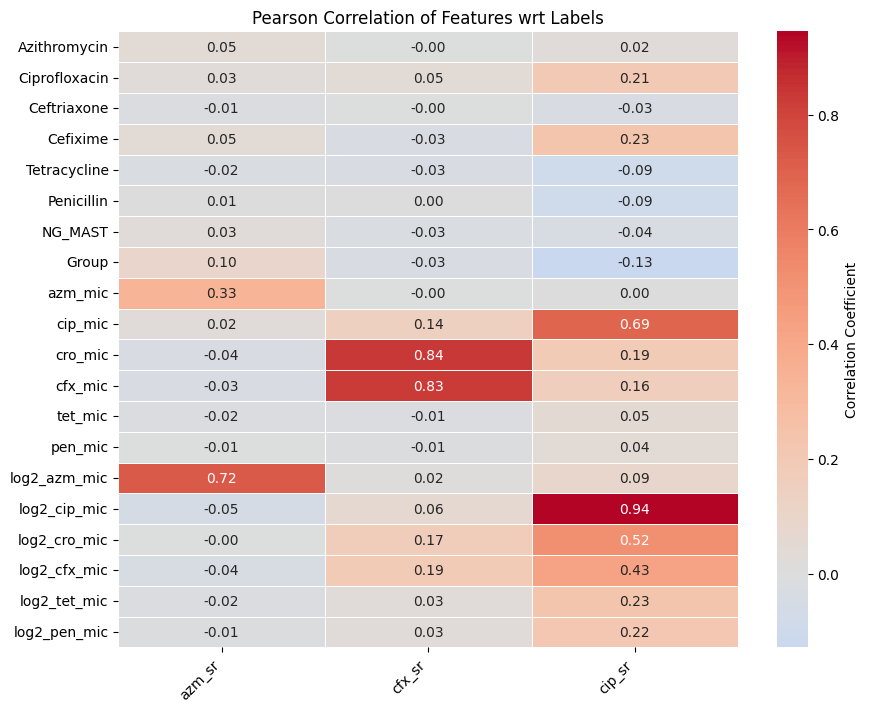
\includegraphics[width=1\textwidth]{figures/corr.png}
                \caption{Correlation analysis.}
                \vspace{-15pt}
            \end{figure}

    \item[6.] Feature Extraction - Based on the correlation matrix generated from previous step and the visualizations beforehand, we extract a list of the most
    impactful features for every target label. This is useful because with a smaller subset of features we can run larger models for the same computational cost. - See table 2.
            \begin{table}[H]
                \centering
                \begin{tabular}{|l|l|l|}
                \hline
                \textbf{Feature}           & \textbf{Correlation} & \textbf{Target} \\ \hline
                Group                      & 0.0955               & azm\_sr         \\ \hline
                azm\_mic                   & 0.3331               & azm\_sr         \\ \hline
                log2\_azm\_mic             & 0.7250               & azm\_sr         \\ \hline
                log2\_cip\_mic             & -0.0515              & azm\_sr         \\ \hline
                cip\_mic                   & 0.1412               & cfx\_sr         \\ \hline
                cro\_mic                   & 0.8370               & cfx\_sr         \\ \hline
                cfx\_mic                   & 0.8258               & cfx\_sr         \\ \hline
                log2\_cip\_mic             & 0.0622               & cfx\_sr         \\ \hline
                log2\_cro\_mic             & 0.1664               & cfx\_sr         \\ \hline
                log2\_cfx\_mic             & 0.1894               & cfx\_sr         \\ \hline
                Ciprofloxacin              & 0.2057               & cip\_sr         \\ \hline
                Cefixime                   & 0.2324               & cip\_sr         \\ \hline
                Tetracycline               & -0.0876              & cip\_sr         \\ \hline
                Penicillin                 & -0.0924              & cip\_sr         \\ \hline
                Group                      & -0.1286              & cip\_sr         \\ \hline
                cip\_mic                   & 0.6896               & cip\_sr         \\ \hline
                cro\_mic                   & 0.1941               & cip\_sr         \\ \hline
                cfx\_mic                   & 0.1630               & cip\_sr         \\ \hline
                log2\_azm\_mic             & 0.0878               & cip\_sr         \\ \hline
                log2\_cip\_mic             & 0.9448               & cip\_sr         \\ \hline
                log2\_cro\_mic             & 0.5225               & cip\_sr         \\ \hline
                log2\_cfx\_mic             & 0.4287               & cip\_sr         \\ \hline
                log2\_tet\_mic             & 0.2316               & cip\_sr         \\ \hline
                log2\_pen\_mic             & 0.2175               & cip\_sr         \\ \hline
                \end{tabular}
                \caption{Impactful features and their correlation with different target variables. Note, "Group" is a feature.}
            \end{table}

    \item[7.] Outlier detection and removal - We visualized the outliers within our data and subsequently remove them. Outliers may give our model a biased perspective on the majority of the data and leads to less accurate predictions. Replacing the outliers maintains the integrity of the dataset while minimizing the impact of extreme values. - See figure 4.
            \begin{figure}[H]
                \centering
                \vspace{-10pt}
                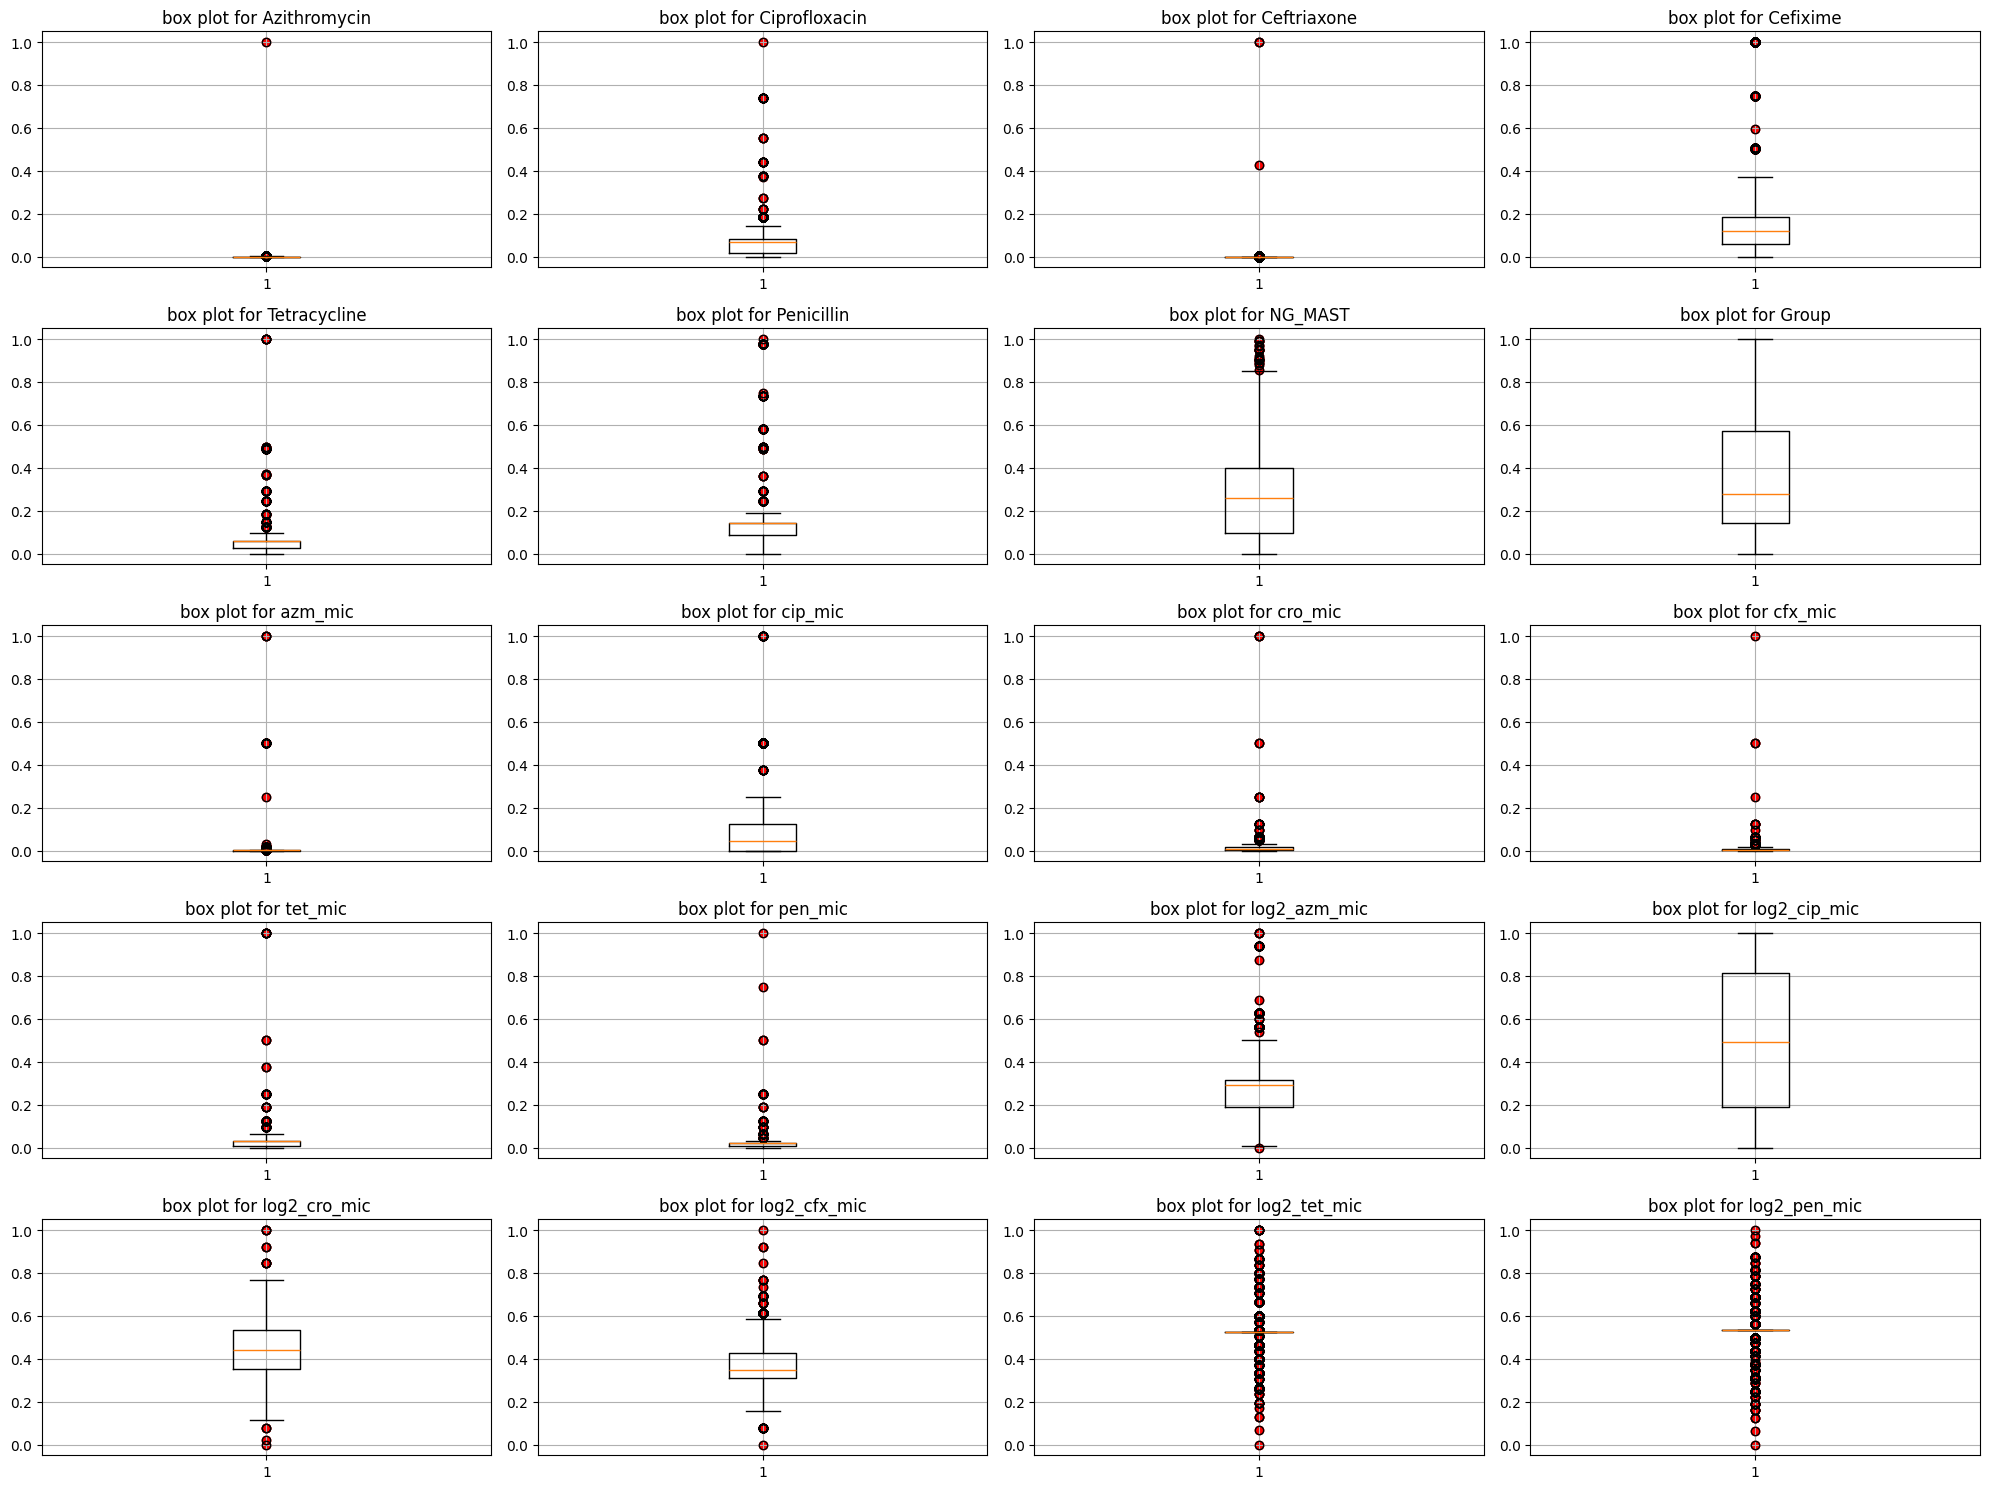
\includegraphics[width=0.7\textwidth]{figures/outlier.png}
                \caption{Outlier analysis.}
                \vspace{-10pt}
            \end{figure}

    \item[8.] Pairwise correlation detection between features - visualize the parwise relationship between each numeric feature to help us identify 
    potential features we can engineer and expose high impact features. See "pairwisefeatures.png". Image too large to embed. 

    \item[9.] Eliminate non intersecting entries between datasets. Each sample will have a total presence for each of the 3 strains we are looking at. The unitig files have binary entries representing whether or not a unitig was present in the sample. Take the sum of each row to get presence of unitigs for each strain for each sample. This simplifies the unitig data files and may help our statistical model identify the relationship between unitigs and a strains resistance to antibiotics.

    \item[10.] Visualize unitig presence, This step helps us get a good perspective on how the unitig presence varies across the sample dataset and its possible distribution. It can help us identify skewness and observe prevalence of different unitigs within the samples providing a clearer picture of the data's characteristics. - see figure 5

        \begin{figure}[H]
                \centering
                \vspace{-10pt}
                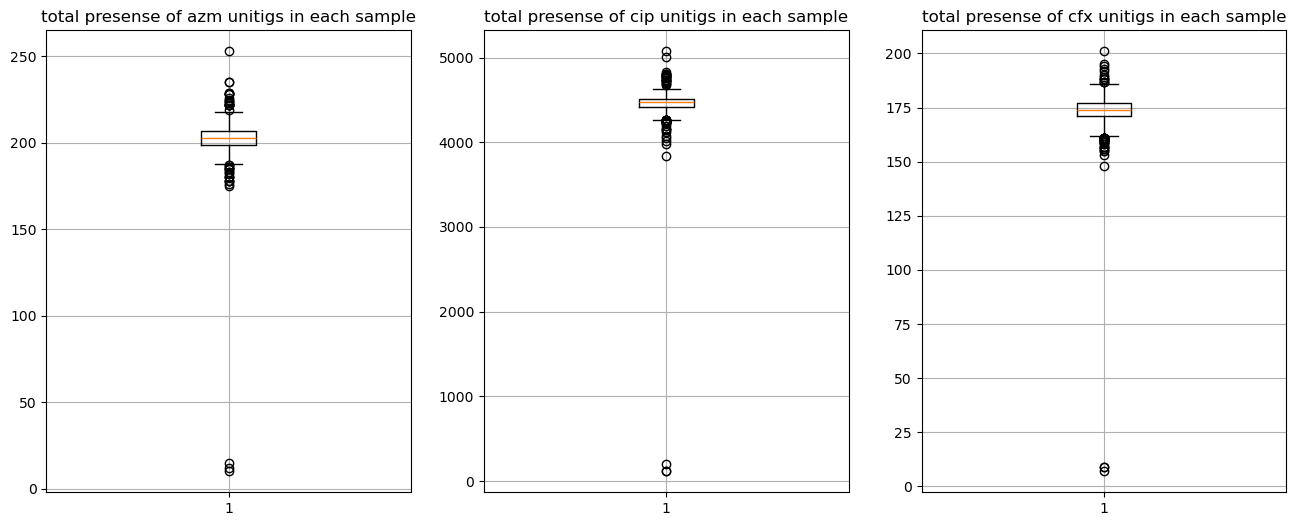
\includegraphics[width=0.7\textwidth]{figures/unitigdis.png}
                \caption{Outlier analysis.}
                \vspace{-10pt}
        \end{figure}

    \item[11.] Evaluate the Mean, Median, Mode, Std, Variance of Unitig Presence. This step provides us with a idea of the typical value and distribution for the unitig presence data. - see table 3.
        \begin{table}[H]
            \centering
            \begin{tabular}{|l|l|l|l|l|l|}
            \hline
            \textbf{Column}       & \textbf{Mean}    & \textbf{Median}  & \textbf{Mode}  & \textbf{Std}     & \textbf{Variance} \\ \hline
            azm presence          & 202.4542         & 203.0            & 204            & 8.8433           & 78.2038           \\ \hline
            cip presence          & 4452.0450        & 4472.0           & 4512           & 168.6345         & 28437.5858        \\ \hline
            cfx presence          & 4452.0450        & 4472.0           & 4512           & 168.6345         & 28437.5858        \\ \hline
            \end{tabular}
            \caption{Summary Statistics for azm, cip, and cfx presence}
        \end{table}

    \item[12.] Visualize distribution of unitig presence. This step gives us a visual representation on how widely the data is distributed across the dataset. It also shows us the density of values within the unitig files - see figure 6
        \begin{figure}[H]
            \centering
            \vspace{-10pt}
            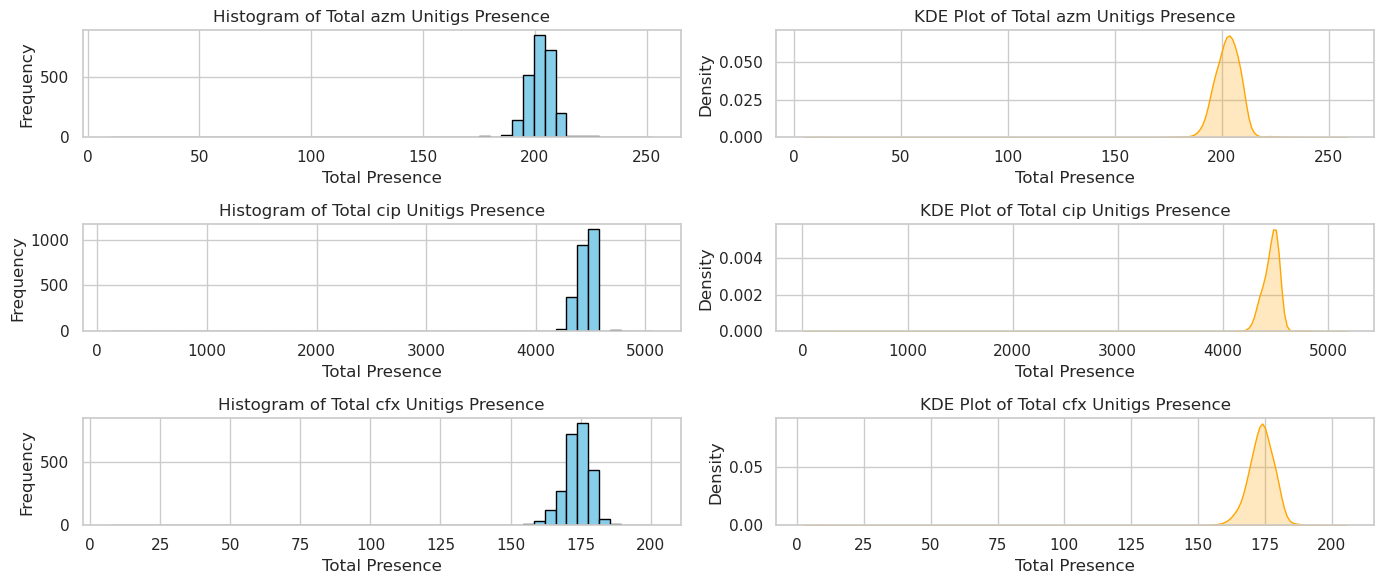
\includegraphics[width=0.7\textwidth]{figures/unitighist.png}
            \caption{Outlier analysis.}
            \vspace{-10pt}
        \end{figure}

    \item[13.] Determine correlation of engineered unitig features to labels by calculating correlation coefficients. This analysis helps identify which unitig features will have a significant relationships to the labels allowing us to assess their predictive relevance. - see figure 7
        \begin{figure}[H]
            \centering
            \vspace{-10pt}
            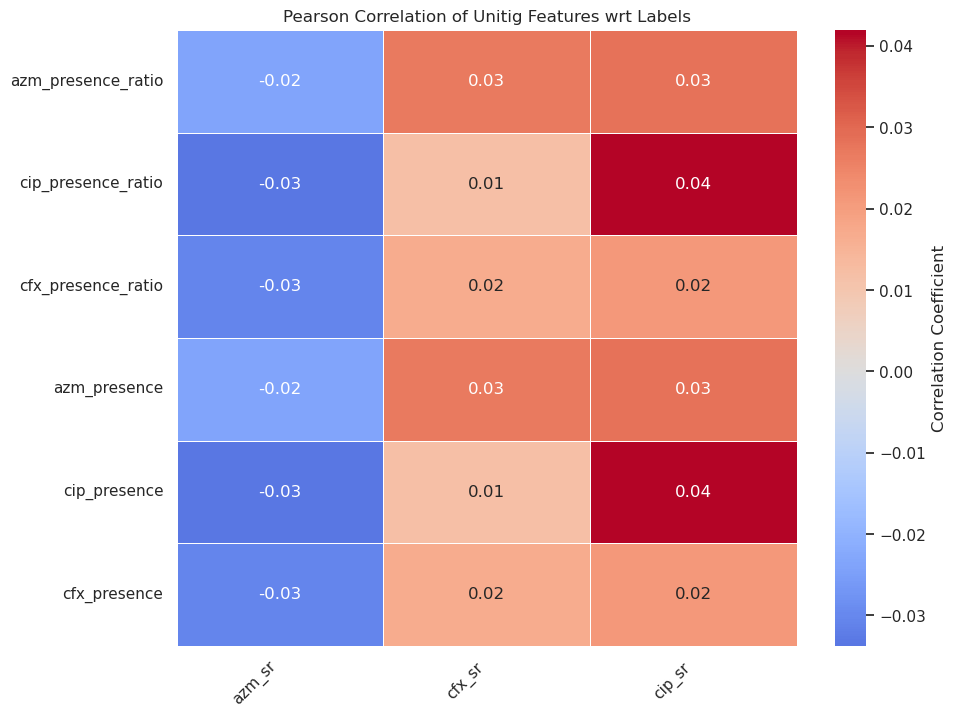
\includegraphics[width=0.7\textwidth]{figures/unitig_corr.png}
            \caption{Outlier analysis.}
            \vspace{-10pt}
        \end{figure}
    \item[14.] Create polynomial features to expose potential nonlinear relationships between existing features and labels. Involves generating new features by raising the original features to a specified power. This can enhance the model's ability to learn more complex patterns and improve predictive performance. - see table 4
        \begin{table}[H]
            \centering
            \begin{tabular}{|c|c|c|c|c|c|c|c|c|}
            \hline
            \textbf{azm\_mic\^{}2} & \textbf{log2\_azm\_mic\^{}2} & \textbf{azm\_presence\^{}2} & \textbf{cip\_mic\^{}2} & \textbf{log2\_cip\_mic\^{}2} & \textbf{cip\_presence\^{}2} & \textbf{cfx\_mic\^{}2} & \textbf{log2\_cfx\_mic\^{}2} & \textbf{cfx\_presence\^{}2} \\ \hline
            1.640527e-07           & 0.083783                      & 0.567139                     & 9.765928e-10            & 0.009855                      & 0.704733                     & 0.000004                 & 0.095175                      & 0.688729                    \\ \hline
            1.640527e-07           & 0.083783                      & 0.560958                     & 1.350796e-02            & 0.242330                      & 0.712201                     & 0.000004                 & 0.095175                      & 0.697311                    \\ \hline
            5.266821e-08           & 0.063883                      & 0.466663                     & 4.334373e-03            & 0.878655                      & 0.561820                     & 0.000018                 & 0.121591                      & 0.566373                    \\ \hline
            1.640527e-07           & 0.068611                      & 0.554810                     & 4.785306e-08            & 0.059880                      & 0.748038                     & 0.000003                 & 0.090796                      & 0.697311                    \\ \hline
            9.765910e-10           & 0.010527                      & 0.560958                     & 9.765928e-10            & 0.009855                      & 0.704394                     & 0.000004                 & 0.095175                      & 0.714635                    \\ \hline
            \end{tabular}
            \caption{Squared values for azm, cip, and cfx features}
        \end{table}
        
    \item[15.] Identify engineered features with a high correlation to the labels. Select features that pass a threshold of correlation. visualize the density and distribution of these features. This helps illustrate the distribution patterns withing the engineered variables and how they vary relative to the labels. - see figure 8

         \begin{figure}[H]
            \centering
            \vspace{-10pt}
            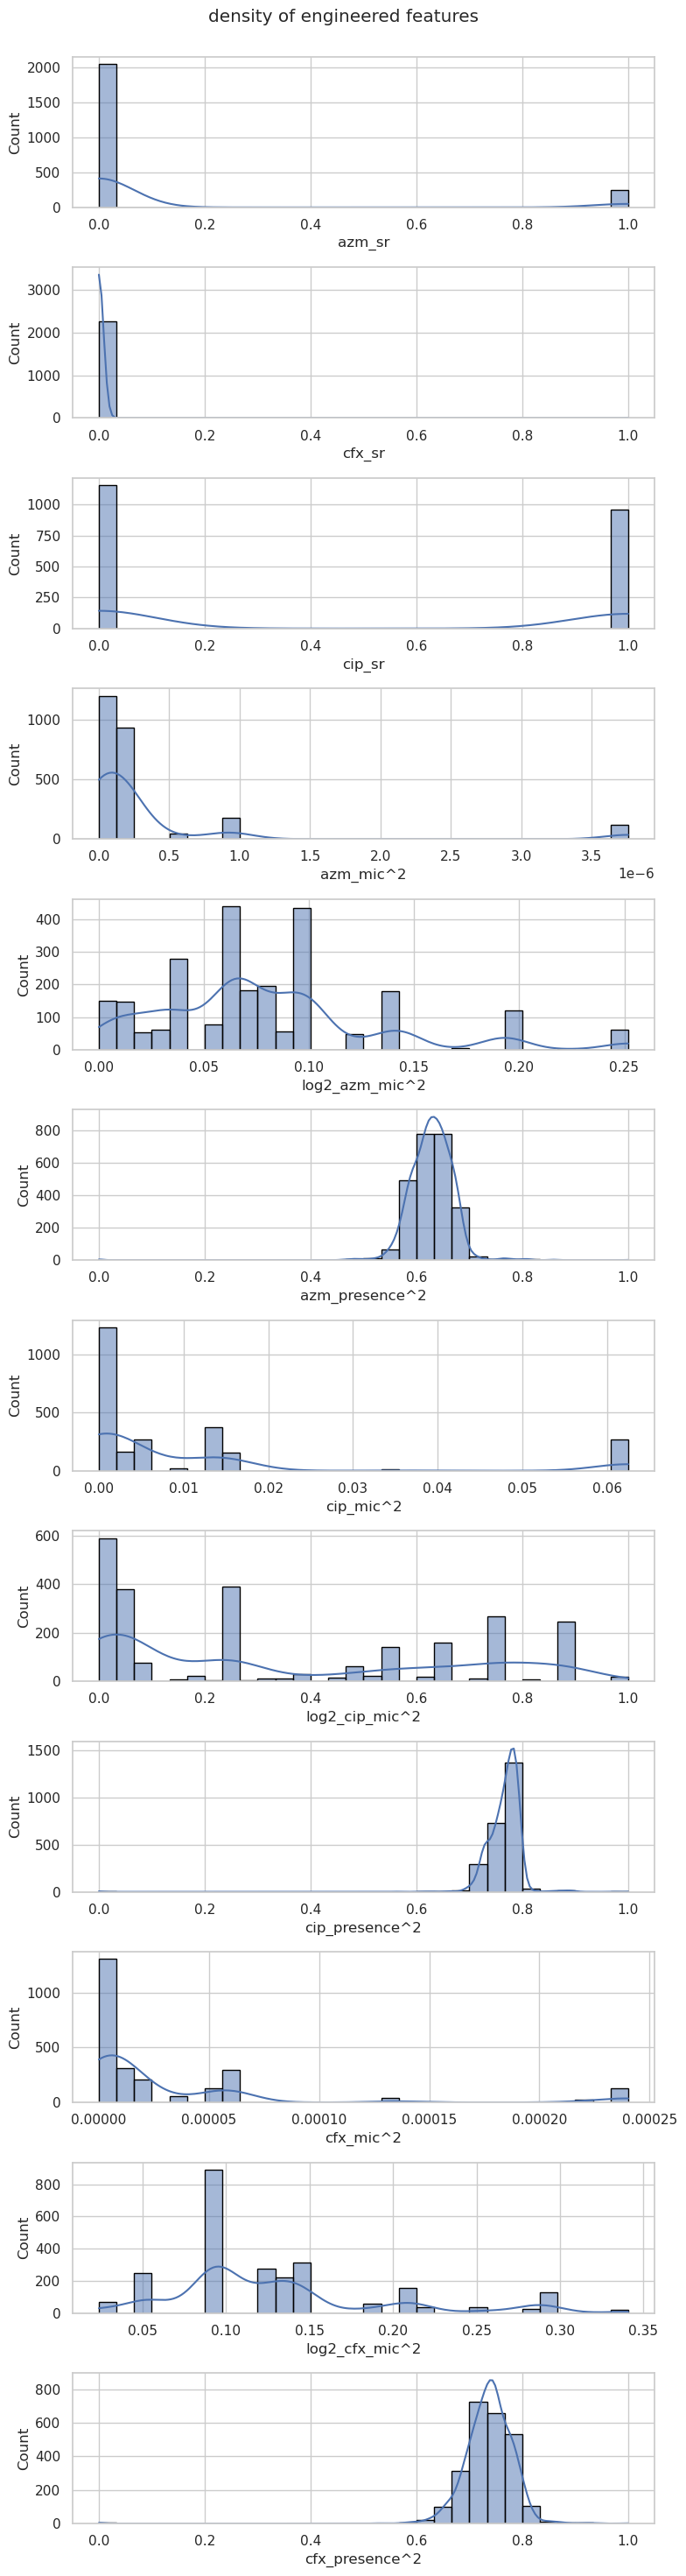
\includegraphics[width=0.7\textwidth]{figures/polydensity.png}
            \caption{Outlier analysis.}
            \vspace{-10pt}
        \end{figure}
    
    \item[16.] Pairwise correlation detection between polynomial features - visualize the parwise relationship between each engineered polynomial feature to help us identify how strongly they correlate. We can compare this to the raw features to see if relevance was improved by the transformations. See "pairwisefeatures.png". Image too large to embed. - see "polypair.png". Image too large to embed.
        



\end{itemize}



\end{document}

